\documentclass[aspectratio=169,11pt]{beamer}

\usetheme{metropolis}

\usepackage[T1]{fontenc}
\usepackage{lmodern}
\usepackage{amsmath,amssymb,bm}
\usepackage{booktabs}
\usepackage{array}
\usepackage{tikz}
\usetikzlibrary{positioning,shapes.geometric,arrows.meta,calc,fit,backgrounds,shadows}
\usepackage{pgfplots}
\pgfplotsset{compat=1.18}
\usepgfplotslibrary{groupplots}
\usepackage{xcolor}

\graphicspath{{../latex_assets/}{latex_assets/}{./latex_assets/}}

\definecolor{HildesheimRed}{RGB}{51,63,156}
\definecolor{PrismBlue}{RGB}{27,94,99}
\definecolor{PrismGreen}{RGB}{46,125,50}
\definecolor{PrismOrange}{RGB}{179,73,31}
\definecolor{PrismRed}{RGB}{51,63,156}
\definecolor{PrismGray}{RGB}{90,90,90}
\definecolor{PrismLightBlue}{RGB}{228,230,247}
\definecolor{PrismLightGreen}{RGB}{232,245,233}
\definecolor{PrismLightOrange}{RGB}{247,229,219}

\metroset{block=fill, progressbar=frametitle, numbering=fraction, sectionpage=progressbar}
\setbeamercolor{palette primary}{bg=HildesheimRed, fg=white}
\setbeamercolor{frametitle}{bg=HildesheimRed, fg=white}
\setbeamercolor{progress bar}{fg=HildesheimRed, bg=PrismGray!25}
\setbeamercolor{alerted text}{fg=HildesheimRed}
\setbeamercolor{block title alerted}{bg=HildesheimRed!85!black, fg=white}
\setbeamercolor{block body alerted}{bg=HildesheimRed!8, fg=black}
\setbeamercolor{block title}{bg=PrismGray!85!black, fg=white}
\setbeamercolor{block body}{bg=PrismGray!8, fg=black}
\setbeamertemplate{navigation symbols}{}
\setbeamerfont{title}{series=\bfseries}

\newcommand{\metric}[2]{\begin{tabular}{c}\textbf{\Large #1}\\[-1mm]{\scriptsize #2}\end{tabular}}
\newcommand{\yes}{\textcolor{PrismGreen}{\textbf{Yes}}}
\newcommand{\partly}{\textcolor{PrismOrange}{\textbf{Partial}}}
\newcommand{\evidence}[1]{\textcolor{HildesheimRed}{\textbf{#1}}}

\title[Advisor Meeting]{Where the Thesis Stands}
\subtitle{\normalsize How it works, what the experiments show, where it succeeds and where it fails}
\author{Brhanu Atsbaha}
\institute{Universität Hildesheim\\[0.15cm]\small \textbf{Advisors:} Prof. Dr. Thomas Mandl \& Shereen Elsayed}
\date{Advisor meeting --- Monday 14 September 2026}


\newcommand{\works}{\textcolor{PrismGreen}{\textbf{Works}}}
\newcommand{\fails}{\textcolor{PrismOrange}{\textbf{Fails}}}
\newcommand{\thin}{\textcolor{HildesheimRed}{\textbf{Thin}}}
\setbeamercolor{block title example}{bg=PrismGreen!80!black, fg=white}
\setbeamercolor{block body example}{bg=PrismLightGreen, fg=black}

\begin{document}

\maketitle

\begin{frame}{What This Meeting Is For}
\begin{columns}[T]
\column{0.55\textwidth}
\small
Since we last spoke I ran every Tier~1 model over the whole $12{,}110$-image corpus for the first time. That changed what I know about my own results.
\vspace{2mm}

This deck is the full picture, in four parts:
\begin{enumerate}\small
  \item \textbf{How the system works} --- the four levels, with the formulas
  \item \textbf{Where it works} --- with the evidence
  \item \textbf{Where it fails} --- with the evidence
  \item \textbf{What I propose} --- and a request
\end{enumerate}

\column{0.42\textwidth}
\begin{block}{\small The honest summary}
\footnotesize The routing mechanism works and is certified. The explanation I originally gave for \emph{why} it works does not survive testing. Several results are thinner than they looked. I would like four more weeks to fix what is fixable.
\end{block}
\end{columns}
\end{frame}

\section{How the System Works}

\begin{frame}{The Task}
\begin{columns}[T]
\column{0.5\textwidth}
\small
\textbf{Index a $53{,}000$-image historical archive} by object and scene --- with no labelled historical data to train on.
\vspace{2mm}

The hard part is not accuracy. A cataloguing system that is often right but cannot say \emph{when} it is wrong gives a curator no way to spend the one scarce resource: expert attention.
\vspace{2mm}

\textbf{So the thesis measures trust, not detection:} which automatic descriptions can be accepted, and which must go to a person.

\column{0.46\textwidth}
\begin{block}{\small Why this is hard}
\footnotesize A detector trained on modern photographs, then retrained on its own pseudo-labels, looks nearly perfect:
\vspace{1mm}
\begin{center}
$\text{mAP}_{50} = \mathbf{0.989}$ \ \ (vs.\ its teacher)
\vspace{1mm}

$\text{mAP}_{50} = \mathbf{0.1462}$ \ \ (vs.\ a human)
\end{center}
\vspace{1mm}
It learned to agree with its teacher's mistakes. Teacher-referenced evaluation cannot see this.
\end{block}
\end{columns}
\end{frame}

\begin{frame}{Architecture: Three Tiers}
\centering
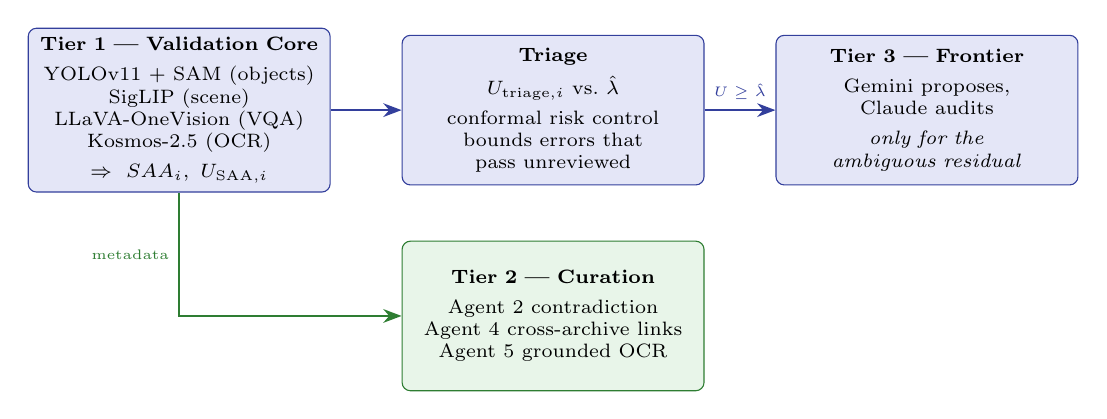
\begin{tikzpicture}[
  node distance=0.5cm and 0.9cm,
  box/.style={draw=HildesheimRed, fill=PrismLightBlue, rounded corners=3pt, align=center, text width=3.6cm, minimum height=1.9cm, font=\scriptsize},
  arrow/.style={->, >=Stealth, thick, HildesheimRed}]
\node[box] (t1) {\textbf{Tier 1 --- Validation Core}\\[1mm] YOLOv11 + SAM (objects)\\ SigLIP (scene)\\ LLaVA-OneVision (VQA)\\ Kosmos-2.5 (OCR)\\[1mm] $\Rightarrow SAA_i,\ U_{\text{SAA},i}$};
\node[box, right=of t1] (tri) {\textbf{Triage}\\[1mm] $U_{\text{triage},i}$ vs.\ $\hat\lambda$\\[1mm] conformal risk control\\ bounds errors that\\ pass unreviewed};
\node[box, right=of tri] (t3) {\textbf{Tier 3 --- Frontier}\\[1mm] Gemini proposes,\\ Claude audits\\[1mm] \emph{only for the}\\ \emph{ambiguous residual}};
\node[box, below=0.7cm of tri, fill=PrismLightGreen, draw=PrismGreen] (t2) {\textbf{Tier 2 --- Curation}\\[1mm] Agent 2 contradiction\\ Agent 4 cross-archive links\\ Agent 5 grounded OCR};
\draw[arrow] (t1) -- (tri);
\draw[arrow] (tri) -- node[above, font=\tiny]{$U\ge\hat\lambda$} (t3);
\draw[arrow, PrismGreen] (t1.south) |- node[pos=0.25, left, font=\tiny]{metadata} (t2.west);
\end{tikzpicture}
\vspace{2mm}

\footnotesize \textbf{Decoupling rule:} Tier~2 enriches metadata \emph{after} routing and never feeds back into trust. Below $\hat\lambda$, images are catalogued automatically; above, they go onward.
\end{frame}

\begin{frame}{The Data}
\centering
\footnotesize
\begin{tabular}{@{}l r l@{}}
\toprule
\textbf{Cohort} & \textbf{Images} & \textbf{Used for} \\
\midrule
$C_0$ full deployment corpus & $12{,}110$ & all signals, full-corpus runs \\
$C_1$ expert-annotated & $801$ & in-sample development \\
Corrected labelled pool & $1{,}250$ & held-out evaluation \\
\quad train / calibration / test & $749$ / $252$ / $249$ & PPN-disjoint: no volume spans a split \\
Negative controls (confirmed) & $319$ & the blind-spot finding \\
Auto-approved audit (in progress) & $45$ of $465$ & direct deployment-risk estimate \\
\midrule
\textbf{Human-labelled, total} & $\mathbf{1{,}580}$ & $\mathbf{13.0\%}$ of the corpus \\
\bottomrule
\end{tabular}
\vspace{3mm}

\begin{alertblock}{\small The number that governs everything else}
\footnotesize $13\%$ of the corpus carries a human label. Every accuracy figure in the thesis is computed on that $13\%$ --- mostly on the $249$-image test partition.
\end{alertblock}
\end{frame}

\section{The Formulation, Level by Level}

\begin{frame}{Level 1 --- Four Signals, Each in $[0,1]$}
\small
Each model emits something incompatible --- boxes, a probability, free text --- so each is mapped to a scalar $A_i \in [0,1]$ per image $i$:
\vspace{1mm}
\begin{align*}
A_i^{\text{object}} &= \min\!\left(\tfrac{n_i^{\text{obj}}}{3},\,1\right) && \text{object count, saturates at } 3 \\[1mm]
A_i^{\text{scene}} &= \text{scene-classifier confidence} && \\[1mm]
A_i^{\text{vlm}} &= \text{VQA object-presence score} && \\[1mm]
A_i^{\text{agree}} &= 1 - \left|A_i^{\text{object}} - A_i^{\text{vlm}}\right| && \text{\emph{derived} --- not a fifth model}
\end{align*}
\vspace{1mm}
\begin{alertblock}{\small Hold onto this}
\footnotesize $A^{\text{agree}}$ is computed \emph{from} two of the others. It is not an independent measurement --- and that turns out to matter more than anything else in the formulation.
\end{alertblock}
\end{frame}

\begin{frame}{Variable Reference I --- The Signals a Model Produces}
\tiny
\begin{center}
\renewcommand{\arraystretch}{0.92}
\begin{tabular}{@{}p{1.6cm} p{2.7cm} p{3.5cm} p{4.2cm}@{}}
\toprule
\textbf{Variable} & \textbf{Which model} & \textbf{Raw output} & \textbf{Reduced to a scalar by} \\
\midrule
$A^{\text{object}}_i$ &
\emph{Intended:} YOLOv11-seg + SAM. \textbf{Actually: the VQA pass} &
\emph{Intended:} boxes, masks, class scores. \emph{Actual:} an integer object count $k$ &
$\min(k/3,\,1)$ --- saturates at $k\!\ge\!3$, so it takes only $\{0,\tfrac13,\tfrac23,1\}$ \\
\addlinespace
$A^{\text{scene}}_i$ &
SigLIP so400m, zero-shot over 5 scene prompts &
Confidence for the best-matching scene category &
Clipped to $[0,1]$. Takes only $\{0.5,\,1\}$ on this corpus \\
\addlinespace
$A^{\text{vlm}}_i$ &
LLaVA-OneVision 7B, VQA &
Free-text answer naming objects present &
Binary object-presence score $\{0,1\}$ \\
\addlinespace
$A^{\text{ocr}}_i$ &
Kosmos-2.5, grounded OCR &
Markdown text, each string tied to a region &
$\min(\ell/80,\,1)$, $\ell$ = characters. Measures \emph{how much} text, not whether it is right \\
\addlinespace
$A^{\text{agree}}_i$ &
\textbf{No model} --- arithmetic on two rows above &
--- &
$1-\left|A^{\text{object}}_i - A^{\text{vlm}}_i\right|$ \\
\bottomrule
\end{tabular}
\end{center}
\vspace{-1mm}
\scriptsize $A^{\text{ocr}}$ feeds the model-level ablation and AWLF, but \emph{not} $SAA$, $U_{\text{SAA}}$ or triage.
\end{frame}

\begin{frame}{Variable Reference II --- What Is Computed From Them}
\tiny
\begin{center}
\renewcommand{\arraystretch}{0.92}
\begin{tabular}{@{}p{1.9cm} p{3.1cm} p{3.4cm} p{4.2cm}@{}}
\toprule
\textbf{Variable} & \textbf{Name} & \textbf{Definition} & \textbf{What it is for} \\
\midrule
$SAA_i$ & Scene-Aware Agreement & $0.6A^{\text{obj}}+0.2A^{\text{scn}}+0.2A^{\text{vlm}}$ & \textbf{Level 2}: decides \emph{what} is in the image. $\ge0.5 \Rightarrow$ scene present \\
\addlinespace
$U_{\text{SAA},i}$ & Disagreement proxy & $\operatorname{std}$ of the four signals, ddof$=1$ & \textbf{Level 3}: decides whether to \emph{trust} the Level-2 answer \\
\addlinespace
$\bar c_i$ & Mean agent confidence & $\tfrac14\sum_j a_{ij}$ over the four & Low mean $=$ nothing convincing found \\
\addlinespace
$U_{\text{triage},i}$ & Triage score & $0.6\,U_{\text{SAA},i}+0.4(1-\bar c_i)$ & \textbf{Level 4}: decides \emph{who sees} the image \\
\addlinespace
$E_i$ & Error indicator & $\mathbb{I}[\,\text{prediction} \neq \text{human label}\,]$ & The target every evaluation scores against \\
\addlinespace
$L_i(\lambda)$ & Conformal loss & $E_i \cdot \mathbb{I}[U_{\text{triage},i} < \lambda]$ & An error let through \emph{unreviewed} \\
\addlinespace
$\hat R(\lambda)$ & Empirical risk & $\tfrac1n\sum_i L_i(\lambda)$ on calibration & What the guarantee bounds \\
\addlinespace
$\alpha$ & Target risk & institution's choice, e.g.\ $0.05$ & The error rate the archive will accept \\
\addlinespace
$\hat\lambda$ & Conformal threshold & largest $\lambda$ with $\tfrac{n}{n+1}\hat R(\lambda)+\tfrac1{n+1}\le\alpha$ & The auto-approval cut-off. \textbf{0.372} here \\
\addlinespace
$\phi_j$ & Shapley attribution & mean marginal gain over coalitions & Interpretability only --- never a deployed weight \\
\bottomrule
\end{tabular}
\end{center}
\end{frame}

\begin{frame}{Why Each Model Emits a Different Kind of Thing}
\small
The four models are chosen to be \emph{heterogeneous} --- that is the whole premise. Each looks at the image in a way the others cannot, so each emits a different type:
\vspace{1mm}
\begin{center}\scriptsize
\begin{tabular}{@{}l l l@{}}
\toprule
\textbf{Model} & \textbf{Question it answers} & \textbf{Output type} \\
\midrule
YOLOv11-seg + SAM & \emph{Where} are things? & geometry: boxes, masks, class scores --- variable length \\
SigLIP so400m & \emph{What kind} of scene? & a probability vector over a fixed taxonomy \\
LLaVA-OneVision 7B & \emph{What is happening?} & free text --- unbounded natural language \\
Kosmos-2.5 & \emph{What does it say?} & markdown text, each string tied to a region \\
\bottomrule
\end{tabular}
\end{center}
\vspace{1.5mm}
\begin{alertblock}{\small The problem this creates --- and it is the thesis's central one}
\footnotesize You cannot take a standard deviation of \{a set of boxes, a probability, a paragraph, some markdown\}. To measure \emph{disagreement} at all, every output must first be crushed into one comparable number in $[0,1]$. That reduction is Level 1 --- and it is where the heterogeneity that motivates the ensemble gets destroyed.
\end{alertblock}
\end{frame}

\begin{frame}{One Image, Four Raw Outputs}
\scriptsize
\texttt{PPN1756550050/00000047\_1} --- the same image, as each model actually sees it:
\vspace{1mm}
\begin{block}{\scriptsize 1. Detector --- geometry}
\tiny\texttt{n\_box: 2 \ \ conf\_mean: 0.9077 \ \ conf\_max: 0.9196 \ \ n\_labels: 1 \ \ labels: ['person']}
\end{block}
\vspace{-1.5mm}
\begin{block}{\scriptsize 2. Scene classifier --- a distribution over five categories}
\tiny\texttt{\{teaching 0.0028, family 0.0105, playing 0.0150, landscape 0.1681, \textbf{drawing 0.8036}\}}
\end{block}
\vspace{-1.5mm}
\begin{block}{\scriptsize 3. VLM --- free text}
\tiny\emph{``A black and white illustration of a man with a gun and a bunch of animals.''} / \emph{``...a black and white silhouette of a rural or pastoral scene...''} / \texttt{yes} / \texttt{outdoor}
\end{block}
\vspace{-1.5mm}
\begin{alertblock}{\scriptsize 4. OCR --- text tied to regions, here degenerate}
\tiny\texttt{\# 2017 \textbackslash n \#\# 2017 \textbackslash n \#\#\# 2017 \textbackslash n \#\#\# 2017 \textbackslash n \#\#\# 2017 ...} \ (repeated 17 times)
\vskip 1pt
\normalsize\textbf{\scriptsize This is the Kosmos degeneracy in the wild} --- $919$ characters of fluent markdown containing no readable inscription. $A^{\text{ocr}} = \min(919/80,1) = \mathbf{1.0}$, the maximum. A length-based signal scores fabrication highest.
\end{alertblock}
\end{frame}

\begin{frame}{The Mapping to $[0,1]$ --- and What Each One Destroys}
\scriptsize
\begin{center}
\tiny
\renewcommand{\arraystretch}{0.95}
\begin{tabular}{@{}p{1.3cm} p{3.0cm} p{3.0cm} p{4.7cm}@{}}
\toprule
\textbf{Signal} & \textbf{Mapping} & \textbf{This image} & \textbf{What the reduction throws away} \\
\midrule
$A^{\text{object}}$ & $\min(k/3,\,1)$, $k$ = object count &
detector $k{=}2 \Rightarrow 0.667$; \textbf{deployed used VQA's $k{=}5 \Rightarrow 1.0$} &
\emph{Where} things are, their confidences, their classes. Saturates at $k\!\ge\!3$: 29 boxes and 3 boxes score alike \\
\addlinespace
$A^{\text{scene}}$ & confidence of best category, clipped &
$\max = 0.804 \Rightarrow \mathbf{1.0}$ &
The other four categories and how \emph{peaked} the distribution was. Takes only $\{0.5,1\}$ deployed \\
\addlinespace
$A^{\text{vlm}}$ & objects named? $\Rightarrow \{0,1\}$ &
names a man, a gun, animals $\Rightarrow \mathbf{1}$ &
Everything the sentence said. A paragraph becomes one bit \\
\addlinespace
$A^{\text{ocr}}$ & $\min(\ell/80,\,1)$, $\ell$ = characters &
$\ell{=}919 \Rightarrow \mathbf{1.0}$ &
Whether the text is \emph{correct}, or even real. Volume, not validity \\
\addlinespace
$A^{\text{agree}}$ & $1-|A^{\text{obj}}-A^{\text{vlm}}|$ &
$1-|1-1| = \mathbf{1.0}$ &
Nothing --- it measures nothing. Arithmetic on two rows above \\
\bottomrule
\end{tabular}
\end{center}
\vspace{-1mm}
\begin{alertblock}{\scriptsize The provenance defect, visible on this one image}
\scriptsize \texttt{student\_v3\_count}$=0$ here, as on all $12{,}110$ images, so the fallback substituted VQA's count. VQA said $5$ objects; the detector finds $2$. The deployed vector is $\mathbf{a}=(1,1,1,1)$ --- perfect unanimity, $U_{\text{SAA}}=0$ --- from a count no detector produced.
\end{alertblock}
\end{frame}

\begin{frame}{Where the Signals Come From: One Model, Four Questions}
\small
Every image goes to LLaVA-OneVision with the same four prompts. Different signals are read from different answers:
\vspace{1mm}
\begin{enumerate}\footnotesize\itemsep3pt
  \item \emph{``Identify objects present: person, child, horse, building, weapon, vehicle, tree, clothing, text, animal.''}\\ $\rightarrow$ the object count behind $A^{\text{object}}$ \textbf{and} the presence score $A^{\text{vlm}}$
  \item \emph{``Which scene fits best: teaching, family, playing, landscape, drawing?''}\\ $\rightarrow$ the scene category and its confidence
  \item \emph{``Describe any archival handwriting or text visible.''} $\rightarrow$ Tier 2 OCR agent only
  \item \emph{``List relational triplets in (Subject, Predicate, Object) format.''} $\rightarrow$ downstream enrichment only
\end{enumerate}
\vspace{2mm}
\begin{alertblock}{\small Why question 1 explains most of this talk}
\footnotesize $A^{\text{object}}$ and $A^{\text{vlm}}$ are both read from the \emph{same answer to the same question}. They were never two independent opinions --- which is why $A^{\text{vlm}} = \mathbb{I}[A^{\text{object}}>0]$ holds on all $12{,}110$ images, and why $A^{\text{agree}}$, built from the pair, adds nothing.
\end{alertblock}
\end{frame}

\begin{frame}{Tier 1 Signal Results --- What the Mapping Leaves}
\scriptsize
Across all $12{,}110$ images, this is what each signal actually takes as values:
\vspace{1mm}
\begin{center}
\begin{tabular}{@{}l c c l c c@{}}
\toprule
& \multicolumn{3}{c}{\textbf{Deployed (fallback path)}} & \multicolumn{2}{c}{\textbf{Rebuilt (real inference)}} \\
\cmidrule(lr){2-4}\cmidrule(lr){5-6}
\textbf{Signal} & \textbf{values} & \textbf{mean} & \textbf{the values themselves} & \textbf{values} & \textbf{mean} \\
\midrule
$A^{\text{object}}$ & $4$ & $0.708$ & $0,\ \tfrac13,\ \tfrac23,\ 1$ & $4$ & $0.467$ \\
$A^{\text{agree}}$ & $3$ & $0.824$ & $\tfrac13,\ \tfrac23,\ 1$ & $6$ & $0.719$ \\
$A^{\text{scene}}$ & $\mathbf{2}$ & $0.712$ & $0.5,\ 1$ & $\mathbf{11{,}882}$ & $0.809$ \\
$A^{\text{vlm}}$ & $\mathbf{2}$ & $0.884$ & $0,\ 1$ & $2$ & $0.593$ \\
$A^{\text{ocr}}$ & $80$ & $0.800$ & $\min(\ell/80,1)$, saturated on $68.6\%$ & $79$ & $0.774$ \\
\midrule
$U_{\text{SAA}}$ & $\mathbf{8}$ & --- & the eight states & $\mathbf{11{,}786}$ & --- \\
\bottomrule
\end{tabular}
\end{center}
\vspace{1mm}
\begin{alertblock}{\small Read the $A^{\text{scene}}$ row}
\footnotesize The scene classifier emits a real-valued confidence, and on real inference it takes $11{,}882$ distinct values. Deployed, it took \textbf{two}. The information was there; the pipeline did not carry it. That single row is most of why $U_{\text{SAA}}$ has only eight states.
\end{alertblock}
\end{frame}

\begin{frame}{Levels 2 and 3 --- One Answer, One Measure of Doubt}
\begin{columns}[T]
\column{0.48\textwidth}
\begin{block}{\small Level 2: $SAA$ --- \emph{what} is in the image}
\footnotesize
\[
SAA_i = 0.6\,A_i^{\text{object}} + 0.2\,A_i^{\text{scene}} + 0.2\,A_i^{\text{vlm}}
\]
Scene present $\iff SAA_i \ge 0.5$.\\[1mm]
A weighted \emph{mean} over three signals. Excludes $A^{\text{agree}}$.
\end{block}

\column{0.48\textwidth}
\begin{block}{\small Level 3: $U_{\text{SAA}}$ --- \emph{trust} that answer?}
\footnotesize
\[
U_{\text{SAA},i} = \operatorname{std}\!\left(A^{\text{obj}}_i, A^{\text{agree}}_i, A^{\text{scn}}_i, A^{\text{vlm}}_i\right)
\]
Sample standard deviation, $\text{ddof}=1$.\\[1mm]
A \emph{spread} over four signals. Includes $A^{\text{agree}}$.
\end{block}
\end{columns}
\vspace{2mm}
\begin{center}
\footnotesize Different operators over different signal sets $\;\Rightarrow\;$ \boxed{U_{\text{SAA}} \neq 1 - SAA}
\end{center}
\vspace{1mm}
\footnotesize The original idea: when heterogeneous models \emph{disagree}, the image is uncertain. Level 3 is meant to measure that disagreement.
\end{frame}

\begin{frame}{The Matrix: What $A^{\text{agree}}$ Actually Reduces To}
\begin{columns}[T]
\column{0.5\textwidth}
\small
$A^{\text{object}}$ takes 4 values and $A^{\text{vlm}}$ takes 2, so $A^{\text{agree}}$ has a $4\times2$ table:
\vspace{1mm}
\[
A^{\text{agree}} =
\bordermatrix{
 & A^{\text{vlm}}{=}0 & A^{\text{vlm}}{=}1 \cr
A^{\text{obj}}{=}0        & \mathbf{1}    & 0 \cr
A^{\text{obj}}{=}\tfrac13 & \tfrac23      & \mathbf{\tfrac13} \cr
A^{\text{obj}}{=}\tfrac23 & \tfrac13      & \mathbf{\tfrac23} \cr
A^{\text{obj}}{=}1        & 0             & \mathbf{1} \cr}
\]
\vspace{1mm}
But $A^{\text{vlm}} = \mathbb{I}[A^{\text{object}}>0]$ on \textbf{every one} of $12{,}110$ images --- so only the \textbf{bold} cells ever occur.

\column{0.46\textwidth}
\begin{block}{\small So it collapses to}
\footnotesize
\[
A^{\text{agree}} =
\begin{cases}
1 & \text{if } A^{\text{object}} = 0\\[1mm]
A^{\text{object}} & \text{otherwise}
\end{cases}
\]
\end{block}
\vspace{1mm}
\begin{alertblock}{\small Consequence}
\footnotesize Identical to $A^{\text{object}}$ on $\mathbf{88.4\%}$ of images. On the rest it \emph{jumps to 1} --- exactly where every model reports nothing.
\vspace{1mm}

The ``fourth opinion'' is the object signal counted twice.
\end{alertblock}
\end{columns}
\end{frame}

\begin{frame}{The Matrix of States: Why $U_{\text{SAA}}$ Has Only Eight Values}
\small
The whole signal vector is fixed by the pair $(A^{\text{object}}, A^{\text{scene}})$ --- so there are only $4 \times 2 = 8$ possible states:
\vspace{1mm}
\begin{center}
\footnotesize
\begin{tabular}{@{}cccc c r@{}}
\toprule
$A^{\text{obj}}$ & $A^{\text{agr}}$ & $A^{\text{scn}}$ & $A^{\text{vlm}}$ & $\bm{U_{\text{SAA}}}$ & \textbf{images} \\
\midrule
$0$ & $1$ & $1$ & $0$ & $\mathbf{0.5774}$ & $195$ \\
$0$ & $1$ & $0.5$ & $0$ & $\mathbf{0.4787}$ & $1{,}208$ \\
$\tfrac13$ & $\tfrac13$ & $1$ & $1$ & $0.3849$ & $222$ \\
$\tfrac13$ & $\tfrac13$ & $0.5$ & $1$ & $0.3155$ & $2{,}217$ \\
$1$ & $1$ & $0.5$ & $1$ & $0.2500$ & $2{,}580$ \\
$\tfrac23$ & $\tfrac23$ & $0.5$ & $1$ & $0.2097$ & $969$ \\
$\tfrac23$ & $\tfrac23$ & $1$ & $1$ & $0.1924$ & $565$ \\
$1$ & $1$ & $1$ & $1$ & $0.0000$ & $4{,}154$ \\
\bottomrule
\end{tabular}
\end{center}
\vspace{1mm}
\footnotesize The two \textbf{largest} uncertainty values are both $A^{\text{object}}=0$ rows --- maximum ``doubt'' exactly where the ensemble is most \emph{unanimous}.
\end{frame}

\begin{frame}{A Worked Example: Unanimous, Yet ``Uncertain''}
\small
Image \texttt{PPN1756555435/00000033\_2}. Every model says \emph{nothing is here}:
\vspace{1mm}
\begin{align*}
\mathbf{a} &= (A^{\text{obj}}, A^{\text{agr}}, A^{\text{scn}}, A^{\text{vlm}}) = (0,\ \mathbf{1},\ 0.5,\ 0), \qquad \bar a = 0.375\\[1mm]
(a_j - \bar a) &= (-0.375,\ +0.625,\ +0.125,\ -0.375)\\[1mm]
\textstyle\sum (a_j - \bar a)^2 &= 0.1406 + \underline{\mathbf{0.3906}} + 0.0156 + 0.1406 = 0.6875\\[1mm]
U_{\text{SAA}} &= \sqrt{0.6875/3} = \mathbf{0.4787} \qquad (83\% \text{ of the maximum } 0.5774)
\end{align*}
\vspace{1mm}
\begin{alertblock}{\small The whole problem in one number}
\footnotesize The underlined term is the \emph{derived} one, supplying $0.39$ of $0.69$. The three \emph{measured} signals $(0,\,0.5,\,0)$ sit close together. The uncertainty is produced by the construction, not by models disagreeing.
\end{alertblock}
\end{frame}

\begin{frame}{Level 4 --- Triage, Under a Risk Guarantee}
\begin{columns}[T]
\column{0.5\textwidth}
\small
\textbf{The triage score} combines spread with low confidence:
\[
U_{\text{triage},i} = 0.6\,U_{\text{SAA},i} + 0.4\,(1 - \bar c_i), \quad \bar c_i = \tfrac14\textstyle\sum_j a_{ij}
\]
\textbf{Auto-approve} image $i$ iff $U_{\text{triage},i} < \hat\lambda$.
\vspace{2mm}

\textbf{Conformal risk control} picks $\hat\lambda$ so that the rate of errors approved \emph{without review} stays below $\alpha$:
\[
\hat\lambda = \max\left\{\lambda : \tfrac{n}{n+1}\hat R(\lambda) + \tfrac{1}{n+1} \le \alpha\right\}
\]
with loss $L_i(\lambda) = E_i \cdot \mathbb{I}[U_i < \lambda]$.

\column{0.46\textwidth}
\begin{block}{\small Worked, $\alpha = 0.05$, $n = 252$}
\footnotesize
\[
\tfrac{1}{n+1} = \tfrac{1}{253} = 0.00395
\]
Largest $\lambda$ on the grid still satisfying the bound:
\[
\hat\lambda = \mathbf{0.372}
\]
\end{block}
\vspace{1mm}
\begin{block}{\small Why this matters}
\footnotesize The guarantee is \emph{distribution-free}: it holds whatever score it is given. So it stays valid even though $U_{\text{SAA}}$ turns out not to measure disagreement.
\end{block}
\end{columns}
\end{frame}

\begin{frame}{How It All Works: Two Real Images, End to End}
\scriptsize
\begin{columns}[T]
\column{0.48\textwidth}
\begin{exampleblock}{\scriptsize \texttt{...00000047\_1} --- auto-approved}
\scriptsize
\textbf{T1} objects found, VQA confirms, scene fires, OCR $919$ chars
\[ \mathbf{a} = (1,\ 1,\ 1,\ 1) \]
\textbf{L2} $SAA = \mathbf{1.0} \ge 0.5 \Rightarrow$ scene present \\
\textbf{L3} $U_{\text{SAA}} = \operatorname{std}(1,1,1,1) = \mathbf{0}$ \\
\textbf{L4} $\bar c = 1$, $U_{\text{triage}} = \mathbf{0} < \hat\lambda$ \\
$\Rightarrow$ \textbf{catalogued automatically}
\vskip 2pt
\textbf{T2} adds label \texttt{person} + OCR. Decides nothing.
\end{exampleblock}

\column{0.48\textwidth}
\begin{alertblock}{\scriptsize \texttt{...00000053\_1} --- escalated}
\scriptsize
\textbf{T1} no objects, VQA reports none, scene still fires
\[ \mathbf{a} = (0,\ \mathbf{1},\ 1,\ 0) \]
\textbf{L2} $SAA = \mathbf{0.2} < 0.5 \Rightarrow$ no scene \\
\textbf{L3} $U_{\text{SAA}} = \operatorname{std}(0,1,1,0) = \mathbf{0.5774}$ \\
\textbf{L4} $\bar c = 0.5$, $U_{\text{triage}} = \mathbf{0.5464} \ge \hat\lambda$ \\
$\Rightarrow$ \textbf{sent to a person}
\vskip 2pt
\textbf{But} three of four signals agree nothing is here.
\end{alertblock}
\end{columns}
\vspace{-0.5mm}
\footnotesize Escalated for the right reason --- genuinely hard --- but the \emph{wrong} cause: the uncertainty is manufactured by $A^{\text{agree}}$, not measured from disagreement.
\end{frame}

\section{Where It Works}

\begin{frame}{Works: It Ranks the Pipeline's Errors Well}
\begin{columns}[T]
\column{0.52\textwidth}
\centering
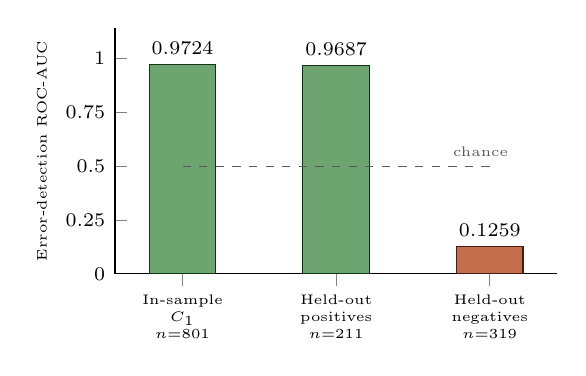
\begin{tikzpicture}
\begin{axis}[ybar, bar shift=0pt, bar width=24pt, width=7.2cm, height=4.7cm, ymin=0, ymax=1.14,
  ylabel={Error-detection ROC-AUC}, ylabel style={font=\tiny},
  symbolic x coords={C1,Held,Neg}, xtick={C1,Held,Neg},
  xticklabels={{In-sample\\$C_1$\\$n{=}801$},{Held-out\\positives\\$n{=}211$},{Held-out\\negatives\\$n{=}319$}},
  x tick label style={font=\tiny, align=center}, tick label style={font=\scriptsize},
  axis lines*=left, enlarge x limits=0.22, nodes near coords,
  every node near coord/.append style={font=\scriptsize\bfseries,/pgf/number format/.cd,fixed,fixed zerofill,precision=4},
  ytick={0,0.25,0.5,0.75,1.0}]
\addplot[fill=PrismGreen!70, draw=PrismGreen!40!black] coordinates {(C1,0.9724) (Held,0.9687)};
\addplot[fill=PrismOrange!80, draw=PrismOrange!40!black] coordinates {(Neg,0.1259)};
\draw[dashed, PrismGray] (axis cs:C1,0.5) -- (axis cs:Neg,0.5) node[pos=0.97, above, font=\tiny, PrismGray]{chance};
\end{axis}
\end{tikzpicture}

\column{0.44\textwidth}
\small
On images that \emph{do} contain a scene, the uncertainty score ranks the pipeline's mistakes almost perfectly --- and that holds on held-out, publication-disjoint data ($0.9687$), not just in-sample.
\vspace{2mm}

\footnotesize The orange bar is the failure mode on true negatives. It is covered on the next section's slides, not hidden here.
\end{columns}
\end{frame}

\begin{frame}{Works: The Risk Guarantee Holds}
\small
Conformal risk control on the corrected, PPN-disjoint test partition ($n=249$):
\vspace{1mm}
\begin{center}
\footnotesize
\begin{tabular}{@{}c c c c c c@{}}
\toprule
$\bm\alpha$ & $\bm{\hat\lambda}$ & \textbf{test risk} & \textbf{bound} & \textbf{auto-approved} & \textbf{error recall} \\
\midrule
$0.01$ & $0.001$ & $0.008$ & \yes & $30.9\%$ & $96.4\%$ \\
$0.02$ & $0.200$ & $0.012$ & \yes & $36.6\%$ & $94.6\%$ \\
$\mathbf{0.05}$ & $\mathbf{0.372}$ & $\mathbf{0.020}$ & \yes & $\mathbf{60.6\%}$ & $\mathbf{91.1\%}$ \\
$0.10$ & $0.372$ & $0.020$ & \yes & $60.6\%$ & $91.1\%$ \\
$0.15$ & $0.537$ & $0.096$ & \yes & $81.5\%$ & $57.1\%$ \\
\bottomrule
\end{tabular}
\end{center}
\vspace{1mm}
\begin{exampleblock}{\small What this buys an archive}
\footnotesize At $\alpha=0.05$: \textbf{$60.6\%$ of images catalogued automatically}, while $91.1\%$ of the pipeline's errors are still caught for review --- a $2.31\times$ efficiency gain over random review, with a stated bound on what slips through.
\end{exampleblock}
\vspace{1mm}
\footnotesize An earlier version reported this bound as \emph{failing}. That was a label-contamination artifact: the negative-control pool was $66.7\%$ mislabelled.
\end{frame}

\begin{frame}{Works: Reproducibility, End to End}
\begin{columns}[T]
\column{0.5\textwidth}
\begin{exampleblock}{\small Everything regenerates from source}
\footnotesize \textbf{$21$ of $21$} verification scripts reproduce their figures exactly.
\vspace{1mm}

Re-executing the fusion stage over all $12{,}110$ images regenerates the committed signal table \textbf{bit-for-bit} --- five columns, maximum difference $0$.
\end{exampleblock}
\vspace{1mm}
\begin{block}{\small The labelled pool is representative}
\footnotesize Because there are only 8 signal states, the labelled pool's mix can be compared directly to the corpus. Total variation distance \textbf{$0.076$}, skewed toward the \emph{harder} states --- so the estimates are, if anything, pessimistic.
\end{block}

\column{0.46\textwidth}
\begin{exampleblock}{\small AWLF v2 meta-classifier}
\footnotesize Error-targeted classifier over agent signals.
\vspace{1mm}
\begin{center}
\begin{tabular}{@{}l r@{}}
In-sample, 5-fold & $0.9896$ \\
Held-out, corrected & $\mathbf{0.8702}$ \\
\end{tabular}
\end{center}
\vspace{1mm}
The earlier $0.6669$ came from the mislabelled pool and is superseded.
\end{exampleblock}
\end{columns}
\end{frame}

\begin{frame}{Works: The Whole Pipeline, Run for Real}
\small
This week: \textbf{all four Tier~1 models on all $12{,}110$ images} --- $4$h$38$m on four A6000s. The first genuinely four-model corpus-wide run.
\vspace{1mm}
\begin{columns}[T]
\column{0.48\textwidth}
\begin{block}{\small Rebuilt, then recalibrated}
\footnotesize Each pipeline with its own calibration, $\alpha=0.05$:
\vspace{1mm}
\begin{center}
\begin{tabular}{@{}l r r@{}}
& \textbf{Deployed} & \textbf{Rebuilt} \\
\midrule
auto-approval & $60.6\%$ & $55.8\%$ \\
error recall & $91.1\%$ & $84.1\%$ \\
risk bound & \yes & \yes \\
\end{tabular}
\end{center}
\end{block}

\column{0.48\textwidth}
\begin{block}{\small At archive scale}
\footnotesize The full $53{,}000$ images would take $\approx\mathbf{21}$ GPU-hours on these cards, producing $\approx36$\,MB.
\vspace{1mm}

\textbf{Compute is not the constraint.} Annotation is.
\end{block}
\end{columns}
\vspace{1mm}
\footnotesize On measured signals the system still works end to end and still certifies --- somewhat less efficiently than the deployed version, not markedly worse.
\end{frame}

\section{Where It Fails}

\begin{frame}{Fails: Disagreement Does Not Beat Plain Confidence}
\begin{columns}[T]
\column{0.5\textwidth}
\small
The thesis's core idea was that \emph{disagreement} between models signals doubt. Tested directly, it does not outperform the simplest baseline --- the pipeline's own confidence, $1 - SAA$.
\vspace{1mm}
\begin{center}
\footnotesize
\begin{tabular}{@{}l r@{}}
\toprule
\textbf{Held-out, $n=249$} & \textbf{ROC-AUC} \\
\midrule
\textbf{Ceiling} (any function) & $\mathbf{0.8871}$ \\
plain confidence & $0.8828$ \\
learned, $A^{\text{agree}}$ dropped & $0.8801$ \\
deployed $U_{\text{SAA}}$ & $0.8600$ \\
\bottomrule
\end{tabular}
\end{center}

\column{0.46\textwidth}
\begin{alertblock}{\small Why no formulation can win}
\footnotesize Only 8 signal states exist, so \emph{any} function of them is constant within a state. Its ranking is fixed by how it orders 8 states. I evaluated all $8! = 40{,}320$ orderings: the best reaches $0.8871$.
\vspace{1mm}

Confidence sits \textbf{$0.0043$} below that ceiling. No weighting, nonlinearity or classifier over these signals can beat it by more.
\end{alertblock}
\vspace{1mm}
\footnotesize Nine formulations were also tried directly. All fell below confidence.
\end{columns}
\end{frame}

\begin{frame}{Fails: And Redesigning the Signals Makes It Worse}
\scriptsize
The obvious repair: stop crushing the outputs. Use the detector's confidence, and the classifier's full distribution over the five scene categories.
\vspace{1mm}
\begin{center}\scriptsize
\begin{tabular}{@{}l r r@{}}
\toprule
& \textbf{Deployed} & \textbf{Redesigned} \\
\midrule
$A^{\text{object}}$: $\min(k/3,1)$ $\rightarrow$ detector max confidence & $4$ values & $\mathbf{8{,}979}$ \\
$A^{\text{scene}}$: binary flag $\rightarrow$ softmax over 5 categories & $2$ values & $\mathbf{11{,}882}$ \\
$A^{\text{vlm}}$: one bit $\rightarrow$ fraction of 10 classes named & $2$ values & $7$ \\
$U_{\text{SAA}}$ & $8$ values & $\mathbf{1{,}247}$ \\
\bottomrule
\end{tabular}
\end{center}
\vspace{-1mm}
\begin{center}\scriptsize
\begin{tabular}{@{}l c c c@{}}
\toprule
\textbf{Signal set} & \textbf{disagreement} & \textbf{confidence} & \textbf{gap (95\% CI)} \\
\midrule
Deployed & $0.8600$ & $0.8828$ & $-0.023$ \\
Redesigned, max softmax & $0.5547$ & $\mathbf{0.8324}$ & $\mathbf{-0.278}$ $[-0.36,-0.20]$ \\
Redesigned, peakedness & $0.6273$ & $\mathbf{0.8430}$ & $\mathbf{-0.216}$ $[-0.29,-0.14]$ \\
\bottomrule
\end{tabular}
\end{center}
\vspace{-2mm}
\begin{alertblock}{\scriptsize The reduction was never the problem}
\scriptsize Given full resolution the gap \emph{widens} from $0.023$ to $0.22$--$0.28$, both intervals below zero. A richer $SAA$ is a better estimate of whether the pipeline is right; its spread is not. \textbf{Not a deployment proposal} --- the redesign is worse in balanced accuracy ($0.66$--$0.68$ vs $0.78$).
\end{alertblock}
\end{frame}

\begin{frame}{Fails: A Shared Blind Spot on True Negatives}
\small
On images a human confirms contain \emph{no} scene, all models agree the image shows something --- and all are wrong. Disagreement stays low exactly where a warning is most needed.
\vspace{1mm}
\begin{center}
\footnotesize
\begin{tabular}{@{}l c c c c@{}}
\toprule
\textbf{Pool} & $\bm n$ & \textbf{errors} & \textbf{ROC-AUC} & \textbf{95\% CI} \\
\midrule
Original held-out & $38$ & $5$ & $0.1152$ & $[0.000,\,0.396]$ \\
New, disjoint annotation pass & $123$ & $27$ & $0.1852$ & $[0.080,\,0.306]$ \\
\textbf{All confirmed negatives} & $\mathbf{319}$ & $\mathbf{50}$ & $\mathbf{0.1259}$ & $[0.062,\,0.196]$ \\
\bottomrule
\end{tabular}
\end{center}
\vspace{1mm}
\begin{alertblock}{\small Replicated --- and partly explained}
\footnotesize The finding survived an independent annotation pass. But a quarter of the gap to chance is \emph{arithmetic}: on a true negative an error needs $SAA\ge0.5$, impossible when $A^{\text{object}}=0$ --- and that is exactly where $A^{\text{agree}}$ jumps to 1. The rest is a genuine failure.
\end{alertblock}
\end{frame}

\begin{frame}{Fails: Two Signals Were Not What They Claimed}
\begin{columns}[T]
\column{0.48\textwidth}
\begin{alertblock}{\small 1. The object signal was a fallback}
\footnotesize The fusion code:
\vspace{1mm}

{\tiny\texttt{if student\_count <= 0:}\\\texttt{\ \ student\_count = vqa\_total\_objects}}
\vspace{1mm}

\texttt{student\_v3\_count} is \textbf{zero on all $12{,}110$ rows}, so the branch always fires. The detector only ever ran on \textbf{$231$} images.
\vspace{1mm}

Confirmed by running both code paths: only the fallback path regenerates the thesis's table.
\end{alertblock}

\column{0.48\textwidth}
\begin{alertblock}{\small 2. The VLM signal is near-constant}
\footnotesize $A^{\text{vlm}}$ = fraction of 4 VQA questions answered in $\ge 3$ words.
\vspace{1mm}

But two questions are yes/no by design:
\vspace{1mm}
\begin{center}
\begin{tabular}{@{}l r@{}}
q0, q1 (descriptive) & $100\%$, $99.9\%$ \\
q2, q3 (yes/no) & $0\%$, $1\%$ \\
\end{tabular}
\end{center}
\vspace{1mm}
So it equals $2/4$ on \textbf{$98.9\%$} of images. It encodes the question format, not the image. \emph{Found only by running the model.}
\end{alertblock}
\end{columns}
\end{frame}

\begin{frame}{Fails --- and the Fix Does Not Rescue It}
\small
The obvious objection: \emph{``your negative result is an artifact of the fallback.''} This week made that testable.
\vspace{1mm}
\begin{center}
\footnotesize
\begin{tabular}{@{}l r r@{}}
\toprule
& \textbf{Deployed (fallback)} & \textbf{Rebuilt (real inference)} \\
\midrule
$U_{\text{SAA}}$ distinct values & $8$ & $\mathbf{11{,}786}$ \\
$A^{\text{vlm}} = \mathbb{I}[A^{\text{object}}>0]$ & $100\%$ & $78.9\%$ \\
disagreement ROC-AUC & $0.8600$ & $0.8098$ \\
confidence ROC-AUC & $0.8828$ & $0.8483$ \\
\bottomrule
\end{tabular}
\end{center}
\vspace{1mm}
\begin{alertblock}{\small Result}
\footnotesize With every signal measured by a real model, the derived term a genuine comparison, and the 8-state discretisation gone --- \textbf{disagreement still trails confidence} ($-0.039$, CI $[-0.083,\,0.005]$). The negative result is not an artifact of the defect.
\end{alertblock}
\end{frame}

\begin{frame}{Fails: Calibration Does Not Transfer Across Publications}
\begin{columns}[T]
\column{0.5\textwidth}
\small
The thesis reports $\text{ECE} < 0.001$ after Platt scaling. That is fitted and scored on a \emph{random} $50\%$ split of $C_1$ --- where pages of the same book fall on both sides.
\vspace{2mm}

On the PPN-disjoint split ($360$ training volumes, $79$ test, \textbf{none shared}):
\vspace{1mm}
\begin{center}
\footnotesize
\begin{tabular}{@{}l r@{}}
\toprule
& \textbf{ECE} \\
\midrule
reported (within-cohort) & $< 0.001$ \\
uncalibrated, disjoint & $0.116$ \\
Platt-scaled, disjoint & $\mathbf{0.109}$ \\
\bottomrule
\end{tabular}
\end{center}

\column{0.46\textwidth}
\begin{alertblock}{\small What it means}
\footnotesize The score \textbf{ranks} errors well across publications ($0.8828$) and is \textbf{not calibrated} across them.
\vspace{1mm}

A monotone recalibration cannot change ranking; what fails to transfer is the map from score to probability.
\vspace{1mm}

An institution relying on the stated \emph{probabilities} must recalibrate on its own holdings.
\end{alertblock}
\end{columns}
\end{frame}

\begin{frame}{Fails: Two Decision Rules, and a Knife-Edge}
\begin{columns}[T]
\column{0.48\textwidth}
\begin{alertblock}{\small A threshold on the seventh decimal}
\footnotesize One state, $(A^{\text{obj}},A^{\text{scn}},A^{\text{vlm}}) = (\tfrac13,\,0.5,\,1)$, lands exactly on the threshold:
\[
0.6\cdot\tfrac13 + 0.2\cdot0.5 + 0.2\cdot1 = 0.5
\]
$A^{\text{object}}$ is \emph{stored} as $0.333333$, so it computes to $\mathbf{0.4999998}$ --- negative by $2\times10^{-7}$.
\vspace{1mm}

This one cell holds \textbf{$2{,}217$ images} ($18.3\%$ of the corpus).
\end{alertblock}

\column{0.48\textwidth}
\begin{alertblock}{\small So two rules coexist}
\footnotesize A stored fusion column holds the exact $0.5$; recomputing from the agent columns gives $0.4999998$.
\vspace{1mm}

They disagree on \textbf{$2{,}217$ images}, and both produced numbers in the thesis:
\vspace{1mm}
\begin{center}
\begin{tabular}{@{}l r@{}}
same weights, same partition & \\
\quad recomputed rule & $70$ errors \\
\quad stored-column rule & $56$ errors \\
\end{tabular}
\end{center}
\end{alertblock}
\end{columns}
\vspace{1mm}
\footnotesize Now fixed in code (threshold moved to $0.55$, in the empty gap; margin $2\times10^{-7}\to0.05$). \textbf{Not yet reconciled in the reported results.}
\end{frame}

\begin{frame}{Thin: The Headline Guarantee Rests on Five Errors}
\begin{columns}[T]
\column{0.5\textwidth}
\small
The certified result --- $60.6\%$ auto-approval, $91.1\%$ recall, risk $0.020 \le 0.05$ --- comes from:
\vspace{2mm}
\begin{center}
\begin{tabular}{@{}l r@{}}
test partition & $249$ images \\
auto-approved & $151$ \\
\textbf{errors among those} & $\mathbf{5}$ \\
\end{tabular}
\end{center}
\vspace{2mm}
Exact $95\%$ interval on that risk:
\[
[\,0.013,\ \mathbf{0.071}\,]
\]

\column{0.46\textwidth}
\begin{alertblock}{\small The problem}
\footnotesize The upper bound, $0.071$, \textbf{exceeds the $\alpha = 0.05$ being certified}.
\vspace{1mm}

Corpus-wide the rule auto-approves $8{,}490$ images. None outside that $249$-image partition has ever been checked.
\end{alertblock}
\vspace{1mm}
\begin{exampleblock}{\small The fix is underway}
\footnotesize Auditing a random sample of auto-approved images: \textbf{$45$ of $465$ done}, $3$ false positives so far. $\sim200$ labels settle it.
\end{exampleblock}
\end{columns}
\end{frame}

\begin{frame}{Tier 2 Agent Results, Against Human Labels}
\scriptsize
Every Tier 2 agent was benchmarked against gold labels collected for this purpose.
\vspace{1mm}
\begin{columns}[T]
\column{0.49\textwidth}
\begin{block}{\scriptsize Agent 2 --- contradiction detection}
\tiny Flags when the VLM names an object the detector did not find. $101$ candidates over $25$ images, judged by a rater.
\vskip 2pt
\textbf{Precision as a hallucination detector: $\mathbf{23.3\%}$} --- the other $76.7\%$ are detector \emph{misses}, not VLM inventions.
\vskip 2pt
Corpus-wide: fires on $71.97\%$ of images, $14{,}933$ flags. Most flagged: \emph{clothing} ($4{,}821$), \emph{text} ($2{,}135$), \emph{tree} ($2{,}076$) --- taxonomy mismatch, since the detector knows 10 classes and the VLM describes freely.
\end{block}

\column{0.49\textwidth}
\begin{block}{\scriptsize Agent 4 --- cross-archive linking}
\tiny $79$ pairs labelled as same-composition / same-style-only / unrelated.
\vskip 2pt
\begin{tabular}{@{}l r r@{}}
\textbf{sim $\ge$} & \textbf{pairs} & \textbf{precision} \\
$0.87$ & $79$ & $0.557$ \\
$0.89$ & $53$ & $0.811$ \\
$0.90$ & $46$ & $0.913$ \\
$\mathbf{0.92}$ & $41$ & $\mathbf{1.000}$ \\
\end{tabular}
\vskip 2pt
Corpus-wide (this week): $2{,}434$ images have a cross-volume candidate at $\ge0.92$; top pairs reach $1.000$ --- duplicate plates in separately catalogued volumes.
\end{block}
\end{columns}
\vspace{1mm}
\begin{alertblock}{\scriptsize Agent 5 --- grounded OCR}
\tiny $53$ rows labelled. Of the \emph{candidate real OCR} bucket ($n{=}40$), only $21$ contain real text: \textbf{precision $0.525$}, median word error rate $100\%$ on the rows with ground truth. Corpus-wide the buckets are $2{,}013$ candidate-real, $6{,}623$ degenerate-repetitive, $3{,}798$ short-or-none. \textbf{Bucket membership is not evidence of legible text.}
\end{alertblock}
\end{frame}

\begin{frame}{Fails: Tier 2 Adds No Corroboration; Tier 3 Untested}
\begin{columns}[T]
\column{0.5\textwidth}
\begin{block}{\small Tier 2, fed from the full re-run}
\footnotesize Agent 2 flags a VLM--detector contradiction on $\mathbf{71.97\%}$ of the corpus --- mostly taxonomy mismatch (\emph{clothing}, \emph{text}, \emph{tree}), not hallucination.
\vspace{1mm}

Where do the flags fall?
\vspace{1mm}
\begin{center}
\begin{tabular}{@{}l r@{}}
auto-approved images & $\mathbf{85.0\%}$ flagged \\
escalated images & $41.4\%$ flagged \\
\end{tabular}
\end{center}
\vspace{1mm}
The images the system trusts \emph{most} carry the \emph{most} contradictions.
\end{block}

\column{0.46\textwidth}
\begin{alertblock}{\small What that means}
\footnotesize The decoupling rule works as designed --- Tier~2 cannot influence routing. But it therefore gives the triage decision no support.
\end{alertblock}
\vspace{1mm}
\begin{block}{\small Tier 3}
\footnotesize Gemini + Claude, frontier-only. Needs paid API credit this project does not have. \textbf{Untested, not falsified.} Its load would be $3{,}620$ images.
\end{block}
\end{columns}
\end{frame}

\section{Summary and Proposal}

\begin{frame}{Scorecard}
\centering
\footnotesize
\begin{tabular}{@{}p{6.4cm} c p{5.2cm}@{}}
\toprule
\textbf{Claim} & \textbf{Status} & \textbf{Evidence} \\
\midrule
Ranks errors on scene-positive images & \works & $0.9687$ held-out \\
Risk guarantee holds & \works & bound met at every $\alpha$ \\
Pipeline reproduces end to end & \works & $21/21$; bit-for-bit table \\
Rebuilt pipeline works for real & \works & $55.8\%$ / $84.1\%$, bound met \\
Labelled pool is representative & \works & TVD $0.076$ \\
\midrule
Disagreement beats confidence & \fails & ceiling $0.8871$; confidence $0.8828$ \\
\quad \emph{...even on redesigned signals} & \fails & gap widens to $-0.22$ to $-0.28$ \\
Detects errors on true negatives & \fails & $0.1259$, $n=319$ \\
Signals are what they claim & \fails & object fallback; VLM $2/4$ on $98.9\%$ \\
Calibration transfers & \fails & ECE $0.109$ disjoint \\
One consistent decision rule & \fails & $2{,}217$ images disagree \\
Tier 2 corroborates triage & \fails & flags $85\%$ vs $41\%$ \\
\midrule
Headline risk is securely estimated & \thin & $5$ errors; CI to $0.071$ \\
Tier 3 frontier pair & \thin & untested (no API budget) \\
\bottomrule
\end{tabular}
\end{frame}

\begin{frame}{What the Thesis Actually Contributes}
\begin{columns}[T]
\column{0.48\textwidth}
\begin{exampleblock}{\small A working, certified system}
\footnotesize A triage policy that catalogues most of an archive automatically under a distribution-free bound on the errors that slip through --- verified on held-out publications and reproducible from source.
\end{exampleblock}
\vspace{1mm}
\begin{exampleblock}{\small A bound, not a survey}
\footnotesize Not ``nine formulations failed'' --- a proof that no formulation over these signals can beat confidence by more than $0.0043$.
\end{exampleblock}

\column{0.48\textwidth}
\begin{block}{\small A documented failure of the stated mechanism}
\footnotesize The system works, but not for the reason proposed. Disagreement is not what makes it work, and the thesis shows why --- two defective signals and a derived term counted twice.
\end{block}
\vspace{1mm}
\begin{block}{\small A methodological lesson}
\footnotesize Teacher-referenced evaluation hid a collapse from $0.989$ to $0.146$. A mislabelled pool reversed a finding. Auditing the \emph{inputs}, not just the numbers, is what caught each of them.
\end{block}
\end{columns}
\end{frame}

\begin{frame}{Request: Four More Weeks}
\small
Five experiments still run on the fallback signals: \textbf{AWLF, CRC, Tier~1 ablation, Shapley, spatial meta-learner.}
\vspace{0.5mm}
\begin{center}
\scriptsize
\renewcommand{\arraystretch}{0.95}
\begin{tabular}{@{}c p{5.8cm} p{5.2cm}@{}}
\toprule
\textbf{Week} & \textbf{Work} & \textbf{Deliverable} \\
\midrule
1 & Finish the auto-approved audit ($465$ labels) & Deployment risk to $\pm1.3$ pp, not $5$ errors \\
2 & Reconcile the two decision rules; re-derive error label and calibration & One authoritative results table \\
3 & Recompute the five experiments on the measured signals & Results chapter on real inputs \\
4 & Re-verify; revise affected sections; rebuild defence materials & Final thesis and deck \\
\bottomrule
\end{tabular}
\end{center}
\vspace{-2mm}
\begin{alertblock}{\small Why not just document it}
\footnotesize I could defend now, listing these as limitations --- but I would be defending a guarantee whose interval overruns its own target, on inputs shown to be a fallback. \textbf{These fixes change what I can claim, not only what I disclose.}
\end{alertblock}
\end{frame}

\begin{frame}{Questions for You}
\begin{enumerate}
  \setlength\itemsep{4mm}
  \item \textbf{Is four weeks acceptable?} Or would you prefer I defend now with these documented as limitations?
  \item \textbf{The negative result is the core finding.} Is a thesis whose central mechanism fails --- but is shown to fail rigorously --- the thesis you want me to defend?
  \item \textbf{The two decision rules.} Reconcile them (re-deriving every downstream number), or document and leave?
  \item \textbf{Tier 3.} Is there any budget for frontier API calls, or should it stay formally untested?
  \item \textbf{Scope.} Anything here you would cut rather than extend?
\end{enumerate}
\end{frame}

\begin{frame}[standout]
Thank you
\vspace{4mm}

{\normalsize Detail on any slide is in the thesis (118\,pp) and the formula reference (18\,pp).}
\end{frame}

\end{document}
